%
%  Vincent Yannello
%
\documentclass[12pt,fullpage]{article}
\usepackage{fullpage}
\usepackage{amsmath}
\DeclareMathOperator{\erf}{erf}
\usepackage{psfrag}                                          % LaTeX graphics tool
\usepackage{pslatex}                                         % avoids the default cmr font
\usepackage{graphicx}                                        % graphics package 
\usepackage{epsfig}                                          % figures
\usepackage{hyperref}
\usepackage{color}

\begin{document}

\noindent
{\bf Makeham distribution} (from \color{blue}\url{http://www.math.wm.edu/~leemis/chart/UDR/UDR.html}\color{black})

\noindent
The shorthand $X \sim {\rm Makeham}(\delta,\, \kappa,\, \gamma)$ is used to indicate that the
random variable $X$ has the Makeham distribution with parameters $\delta$, $\kappa$, $\gamma$.
A Makeham random variable $X$ with parameters $\delta$, $\kappa$, and~$\gamma$ has probability density function 
$$
f(x) = \left( \gamma+{\it \delta}\,{{\it \kappa}}^{\kern 0.08 em x} \right) {e^{-\gamma\,x-
{{\it \delta}\, \left( {{\it \kappa}}^{\kern 0.08 em x}-1 \right)/ \ln 
 \left( {\it \kappa} \right) }}} \qquad \qquad x > 0,
$$
for all $\delta> 0$, $\kappa >1$, and $\gamma>0$. 
The Makeham distribution is used to model adult lifetimes by actuaries.
The probability density function with $\delta=1$, $\kappa=2$, and $\gamma=1$ is illustrated below.
{\begin{figure}[h!]
\begin{center}
\psfrag{lab1}{$\delta \kern -0.08 em = \kern -0.08 em  1,\, \kappa \kern -0.08 em  = \kern -0.08 em  2,\, \gamma \kern -0.08 em  = \kern -0.08 em  1$}
\psfrag{labx}{$x$}
\psfrag{labf}{$f(x)$}
\includegraphics[width=3.2in]{MakehamPlot.ps}
\end{center}
\end{figure}}\\
The cumulative distribution function on
the support of $X$ is
$$
F(x) = P(X \le x) = 1 -{e^{-{(\gamma\,x\ln  \left( {\it \kappa} \right) +{\it 
\delta}\,{{\it \kappa}}^{\kern 0.08 em x}-{\it \delta}) / \ln  \left( {\it \kappa}
 \right) }}}  \qquad \qquad x > 0.
$$
The survivor function on the support of $X$ is
$$
S(x) = P(X \ge x) = {e^{-{(\gamma\,x\ln  \left( {\it \kappa} \right) +{\it 
\delta}\,{{\it \kappa}}^{\kern 0.08 em x}-{\it \delta})/\ln  \left( {\it \kappa}
 \right) }}}  \qquad \qquad x > 0.
$$
The hazard function on the support of $X$ is
$$
h(x) = \frac{f(x)}{S(x)} = \gamma+{\it \delta}\,{{\it \kappa}}^{\kern 0.08 em x} \qquad \qquad x > 0.
$$
The cumulative hazard function on the support of $X$ is mathematically intractable.
$$
H(x) = {\frac {\gamma\,x\ln  \left( {\it \kappa} \right) +{\it \delta}\,{
{\it \kappa}}^{\kern 0.08 em x}-{\it \delta}}{\ln  \left( {\it \kappa} \right) }} \qquad \qquad x > 0.
$$
The inverse distribution function, moment generating function and characteristic function of $X$ are mathematically intractable. The population mean, variance, skewness, and kurtosis of $X$ are also mathematically intractable.

%  \vspace{0.1in}

\newpage

\noindent
{\bf APPL verification:}
The APPL statements
\begin{verbatim}
assume(delta > 0);
assume(gamma > 0);
assume(kappa > 1);
X := [[x-> (y+delta*kappa^x)*exp(-y*x - delta*(kappa^x - 1)/ln(kappa))],
      [0,infinity],["Continuous", "PDF"]];
CDF(X);
SF(X);
HF(X);
CHF(X);
\end{verbatim}
verify the cumulative distribution function, survivor function, hazard function, and cumulative hazard function.

\end{document}
